\chapter{Resultados y discusi\'on}
\label{ch:resultadosRadio}

\section{C\'alculo de la exposici\'on}
	
	
	
	\begin{displaymath}
		\begin{aligned}
			{\cal E} (E_\nu) = 2 \pi T A
			\int_{0}^{\infty} 
			\int_{\theta_D^{cut}}^{\theta_D^{max}} 
			\int_{0}^{E_\nu} 
			\int_{0}^{E_\tau} 
			\epsilon (x_d,\theta_D,Ev) 
			\frac{e^{\frac{l(x_d)}{\lambda(E_\tau)}}}{\lambda(E_\tau)}\frac{dl(x_d)}{dx_d}
			P(E_v|E_\tau)\\
			P(E_\tau|E_\nu,\theta_E(\theta_D))
			\sin \theta_D \cos \theta_D
			dE_v dE_\tau  d\theta_D dx_d
		\end{aligned}
	\end{displaymath}
	
	\begin{figure}[h!]
		\begin{center}
			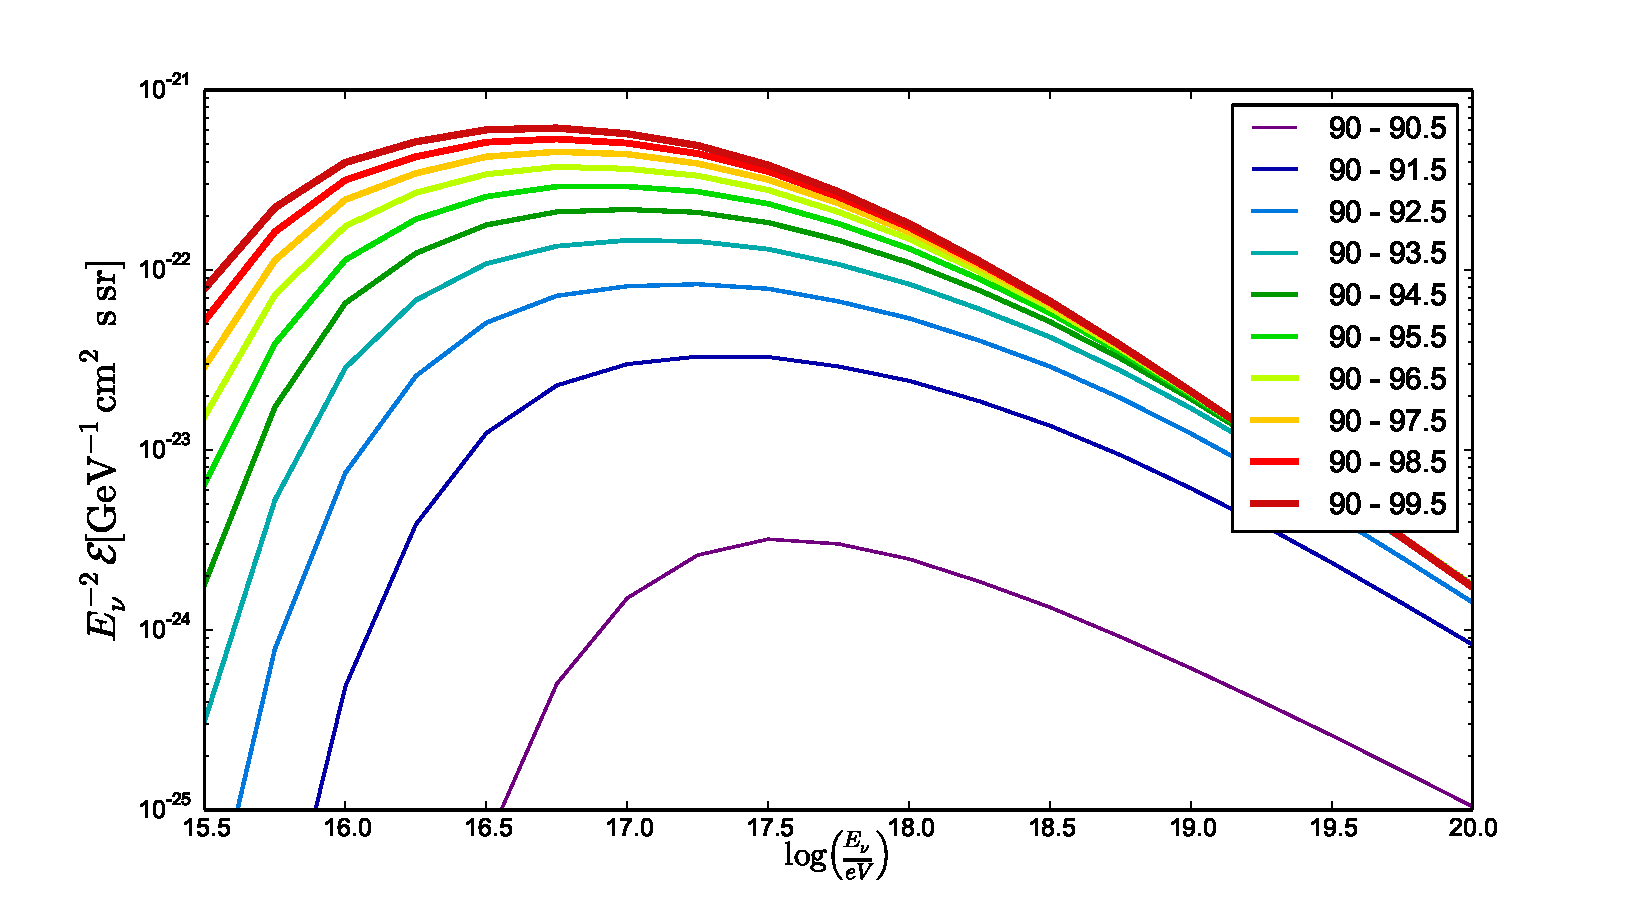
\includegraphics[width=0.9\textwidth]{fig/resultadosRadio/exposureFullEff_thetas}
			\caption{asd}
			\label{fig:}
		\end{center}
	\end{figure}
	
	\begin{figure}[h!]
		\begin{center}
			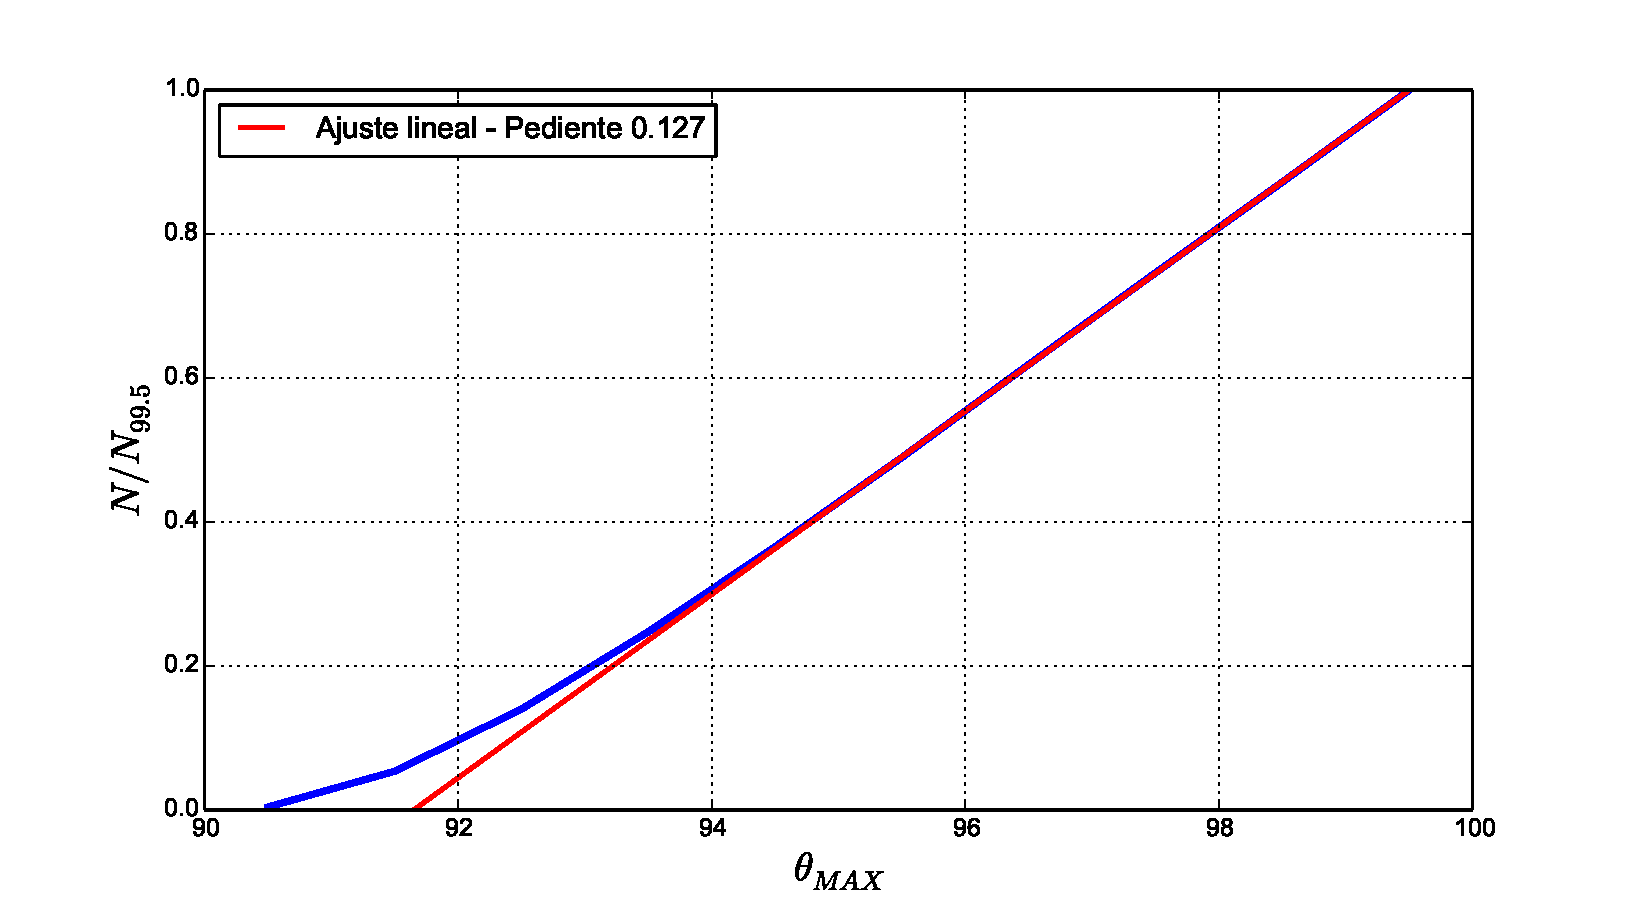
\includegraphics[width=0.9\textwidth]{fig/resultadosRadio/eventGain_thetas}
			\caption{asd}
			\label{fig:}
		\end{center}
	\end{figure}
	
\section{Pesos de las lluvias}

	\begin{figure}[ht!]
		\centering
		\begin{tabular}{cc}
		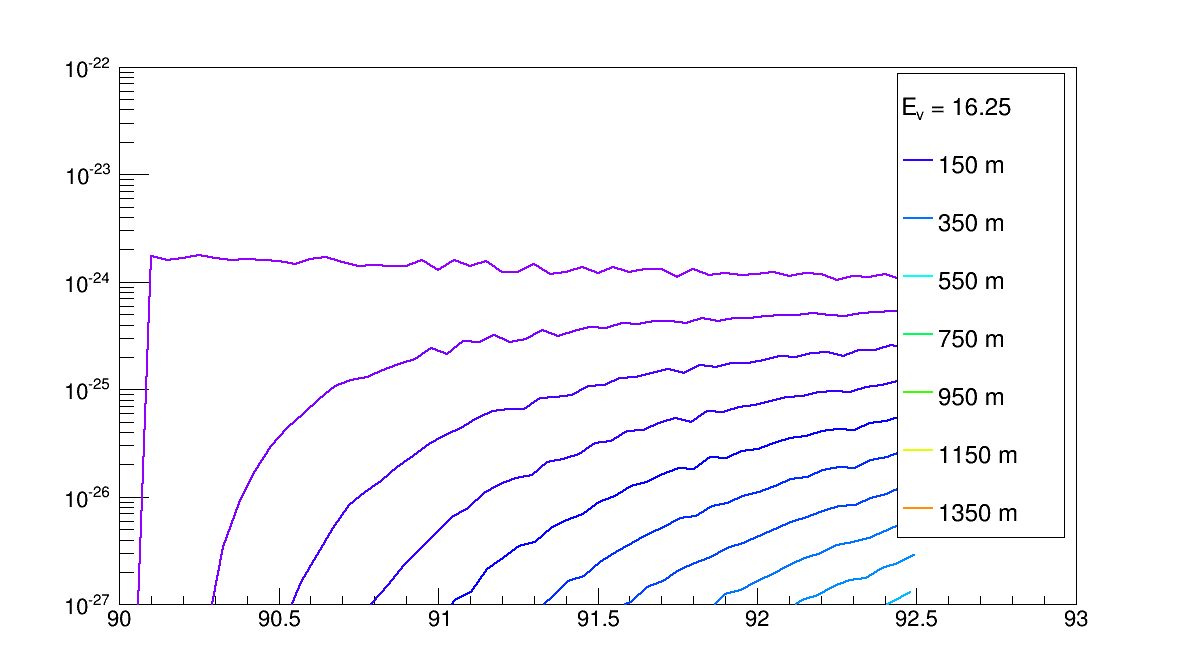
\includegraphics[width=0.45\textwidth]{fig/resultadosRadio/weights16_25.png} &
		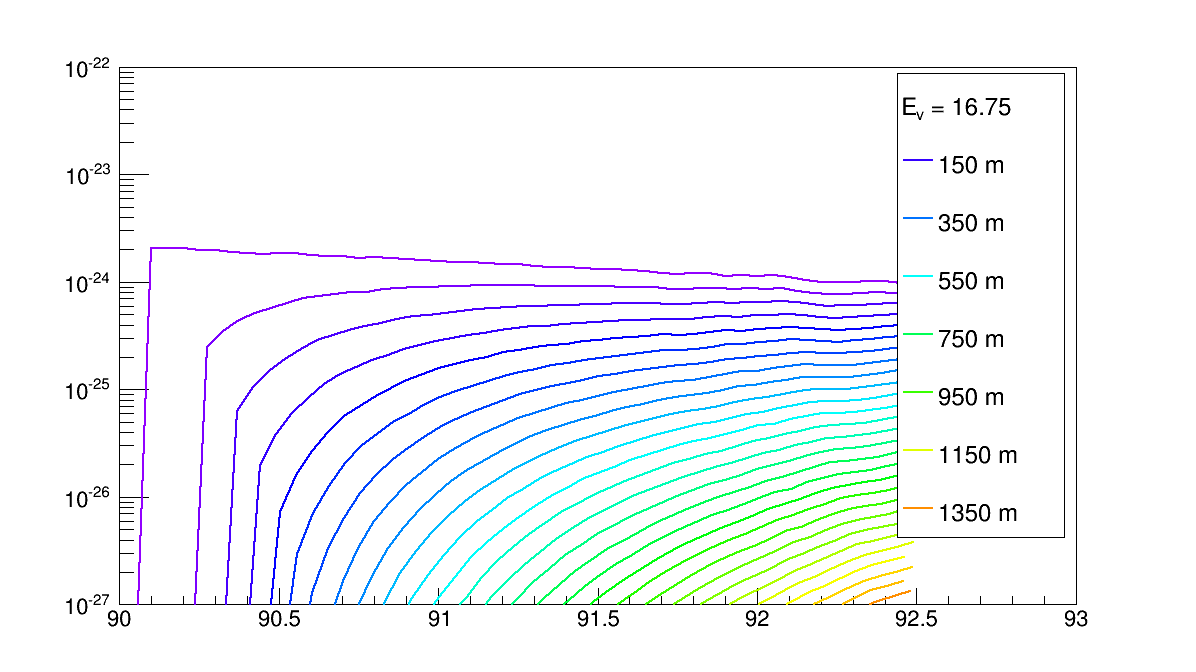
\includegraphics[width=0.45\textwidth]{fig/resultadosRadio/weights16_75.png} \\
		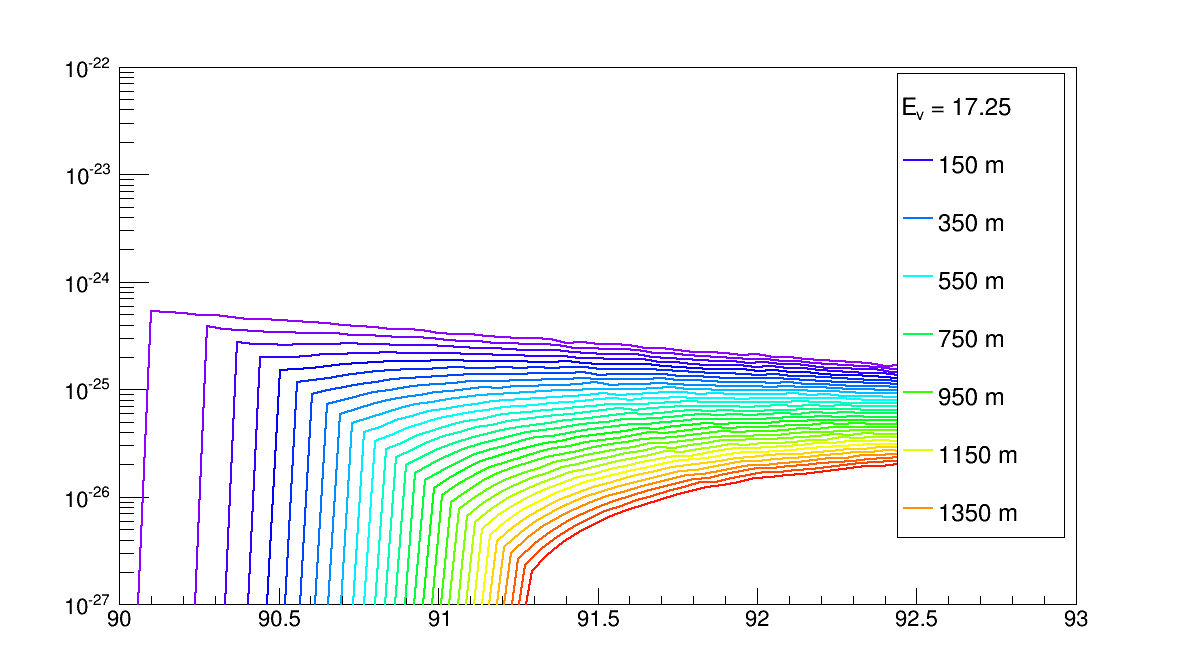
\includegraphics[width=0.45\textwidth]{fig/resultadosRadio/weights17_25.png} &
		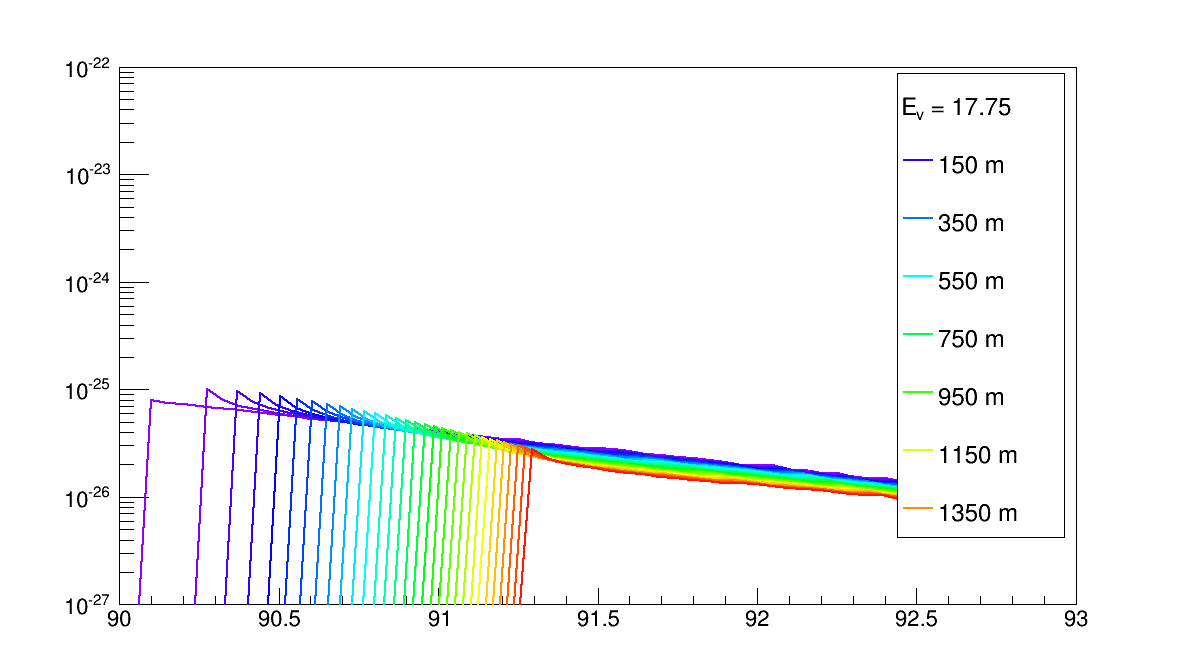
\includegraphics[width=0.45\textwidth]{fig/resultadosRadio/weights17_75.png} \\
		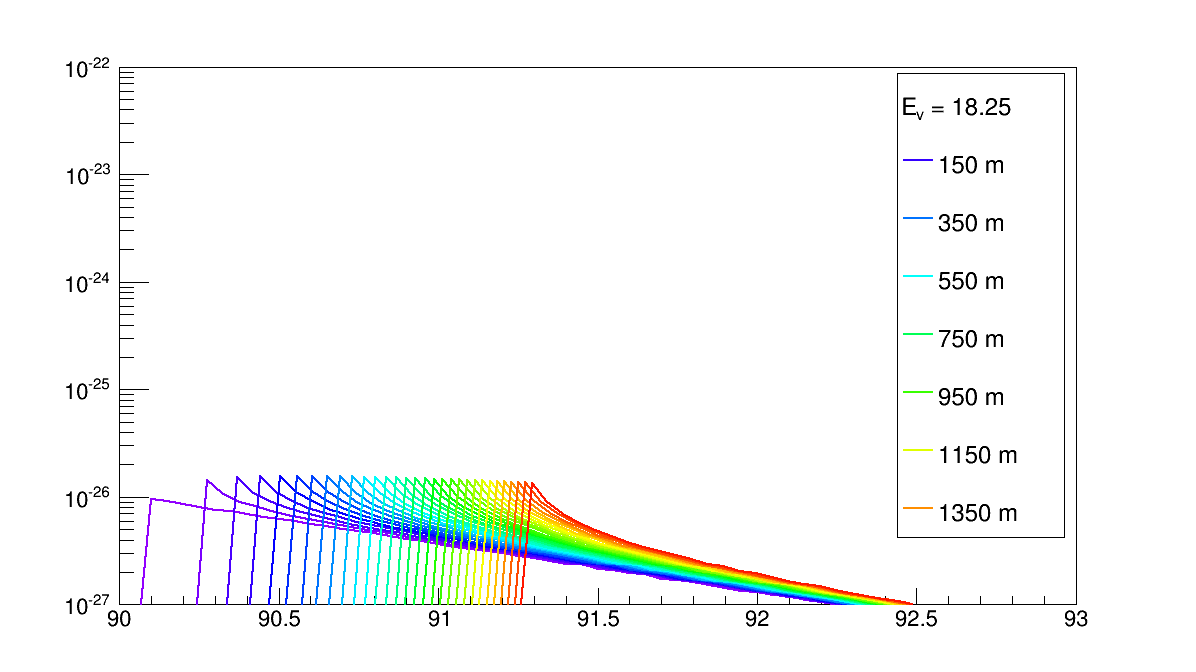
\includegraphics[width=0.45\textwidth]{fig/resultadosRadio/weights18_25.png} &
		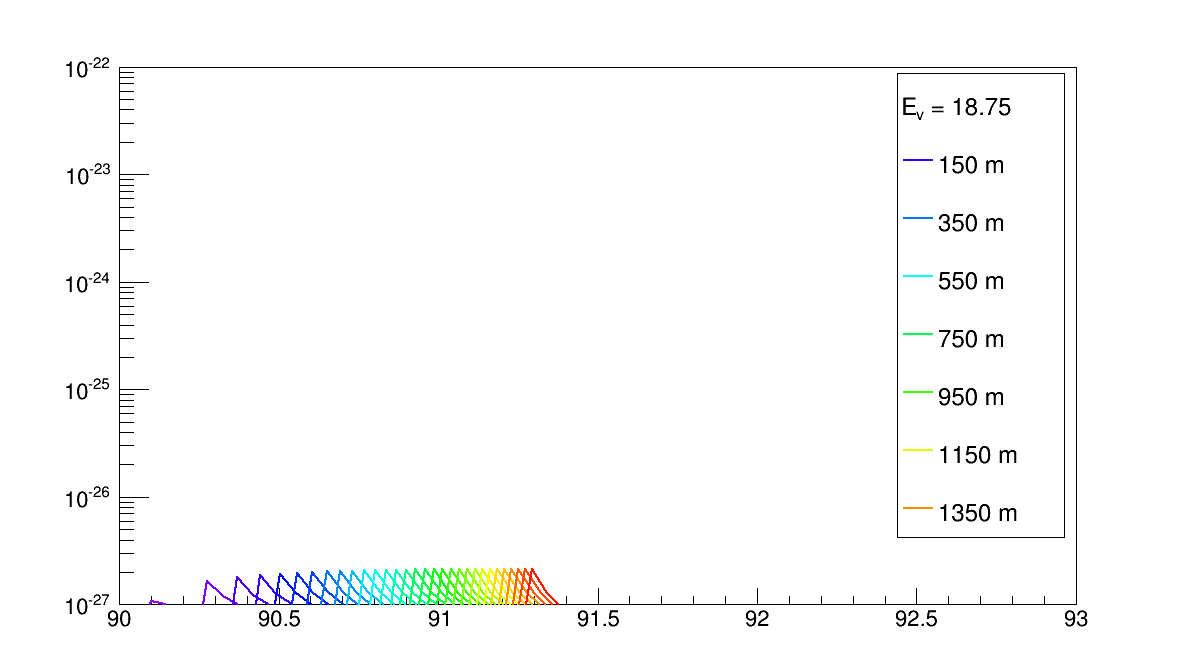
\includegraphics[width=0.45\textwidth]{fig/resultadosRadio/weights18_75.png} \\
		\end{tabular}

		\caption{\label{fig:radioShWeights}
		asd
		}
	\end{figure}
	
	
\section{Eficiencias de trigger e identificaci\'on}
	
	Explicacion dle metodo.
	PLOT PAR DEFINIR TOPOGRAFIAS
	
	\begin{figure}[h!]
		\begin{center}
			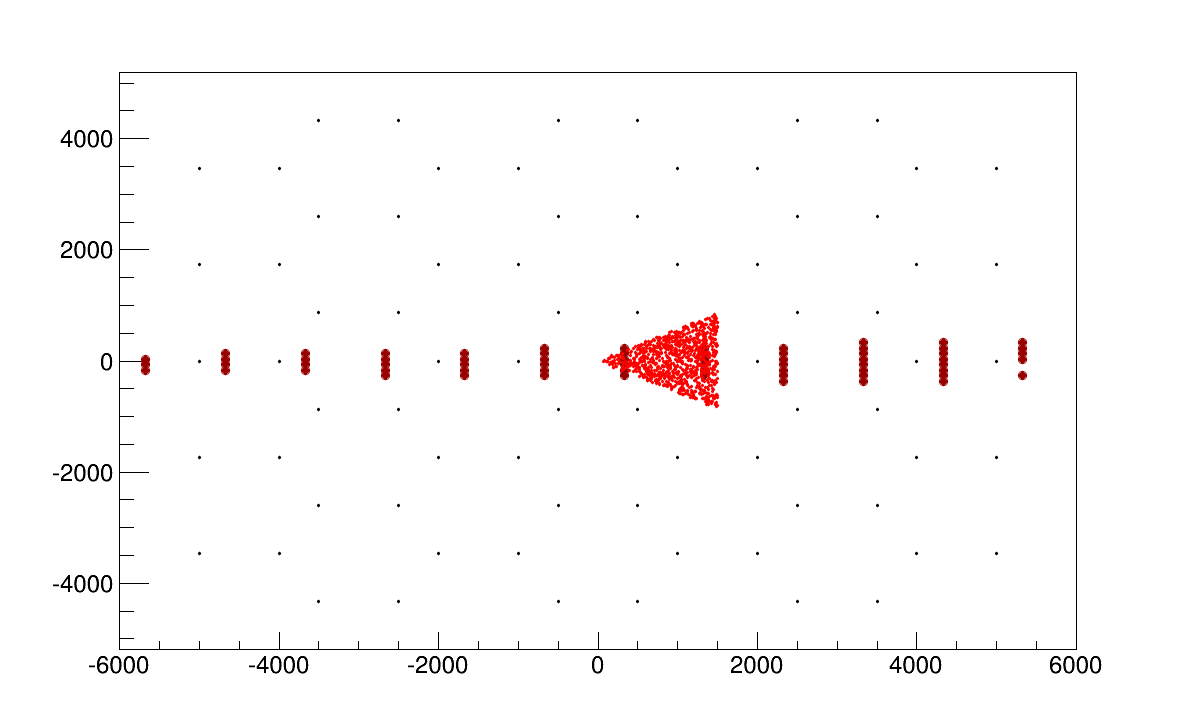
\includegraphics[width=0.9\textwidth]{fig/resultadosRadio/17_00_89_90_00_00_00000_01238_60}
			\caption{asd}
			\label{fig:}
		\end{center}
	\end{figure}
	
	definicion del threshold
	
	descarte del canal muonico
	
	reescaleo por identificacion
	
	\begin{figure}[h!]
		\begin{center}
				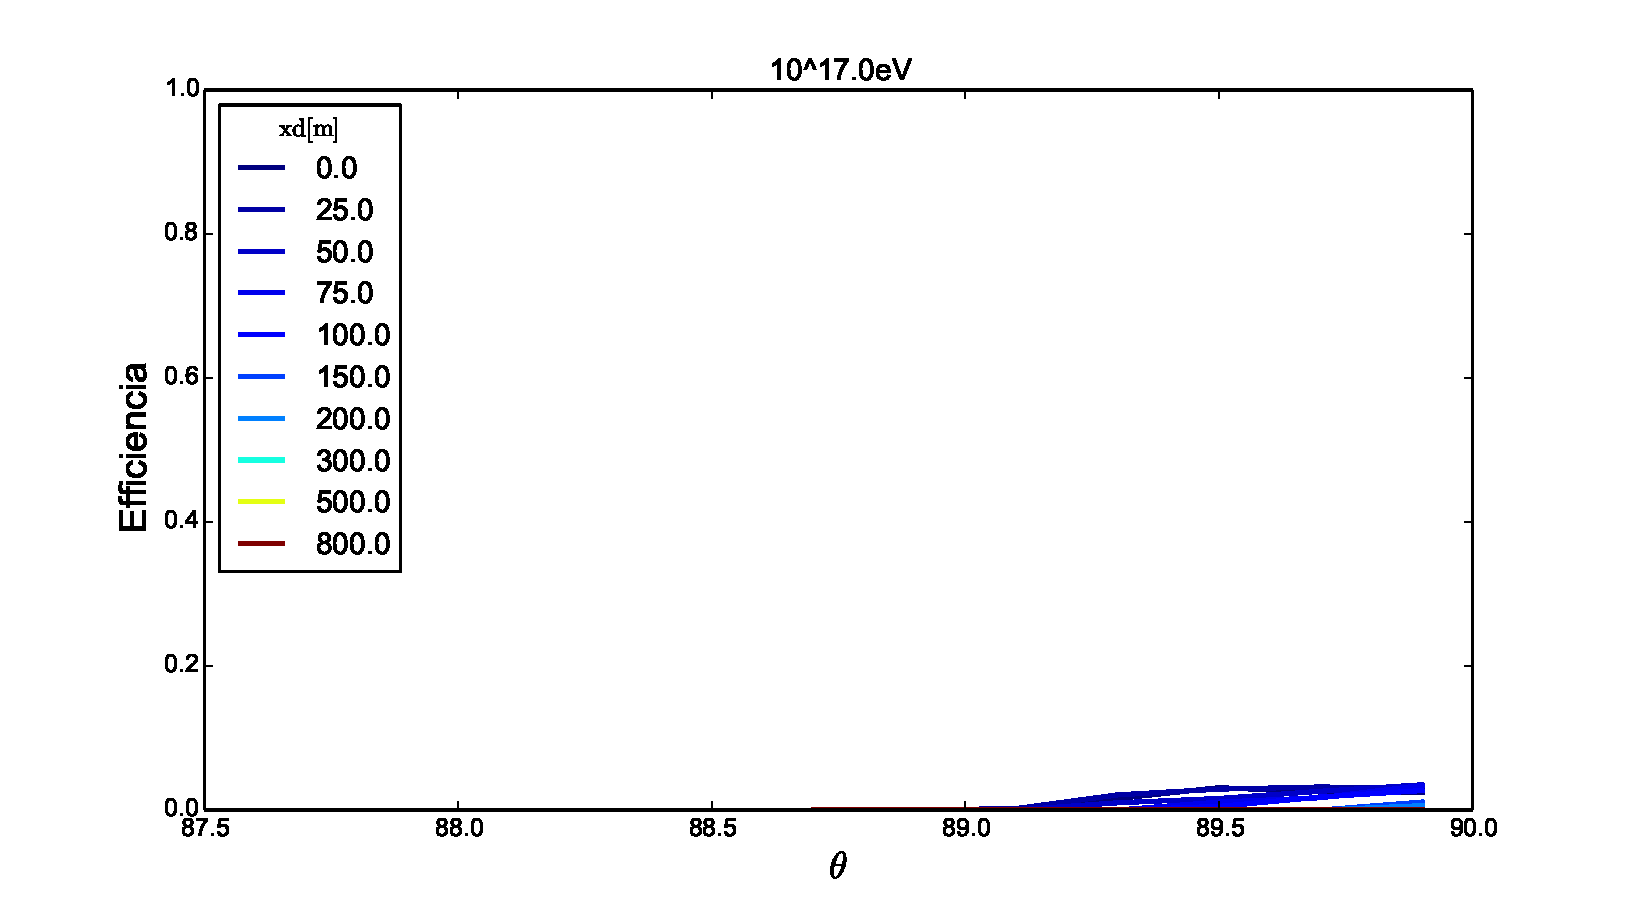
\includegraphics[width=0.9\textwidth]{fig/resultadosRadio/eff75_0_4_0_1500_0_1500_0_60_0_1_0_17_0_m2.pdf} 
				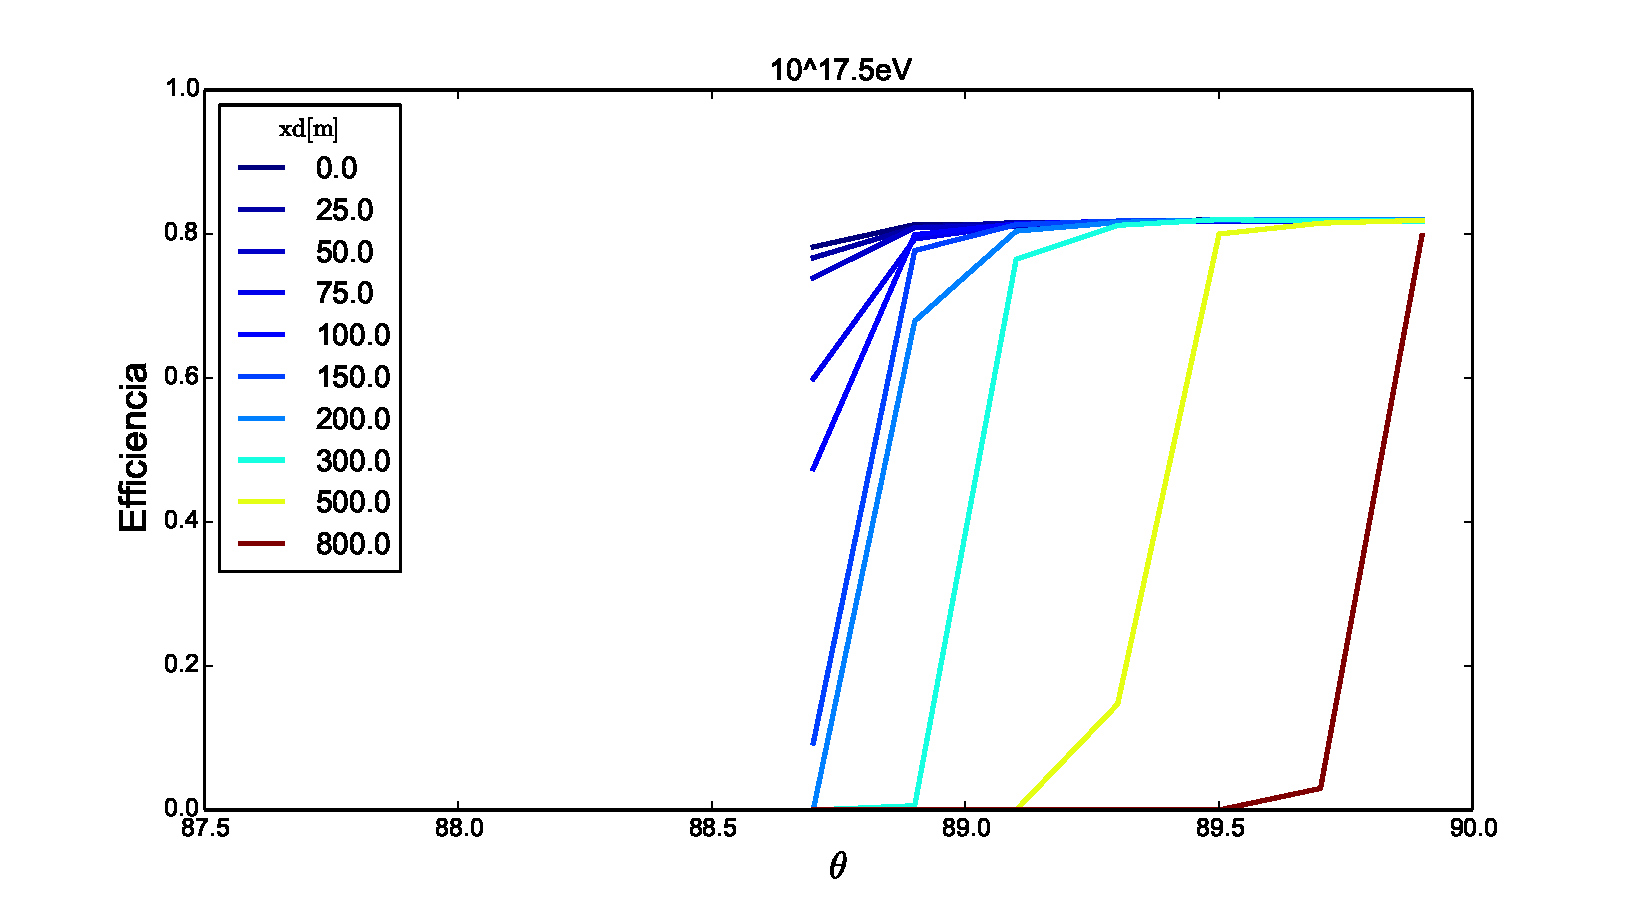
\includegraphics[width=0.9\textwidth]{fig/resultadosRadio/eff75_0_4_0_1500_0_1500_0_60_0_1_0_17_5_m2.pdf}
				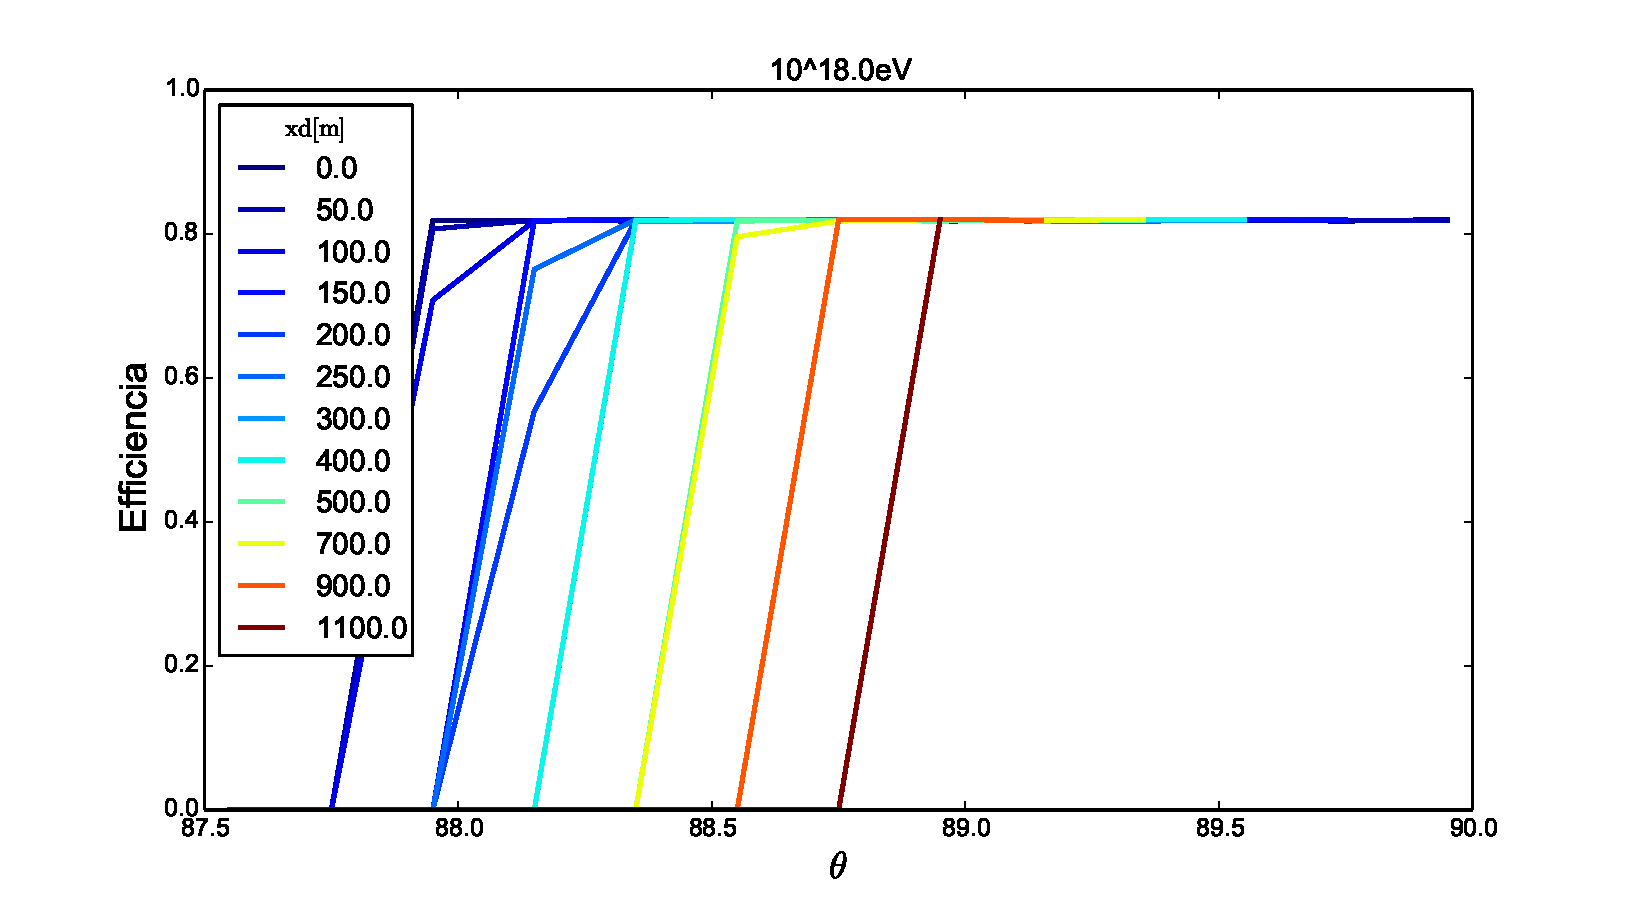
\includegraphics[width=0.9\textwidth]{fig/resultadosRadio/eff75_0_4_0_1500_0_1500_0_60_0_1_0_18_0_m2.pdf}
			\caption{asd}
			\label{fig:}
		\end{center}
	\end{figure}
	
	\begin{figure}[h!]
		\begin{center}
% 		\begin{ta
			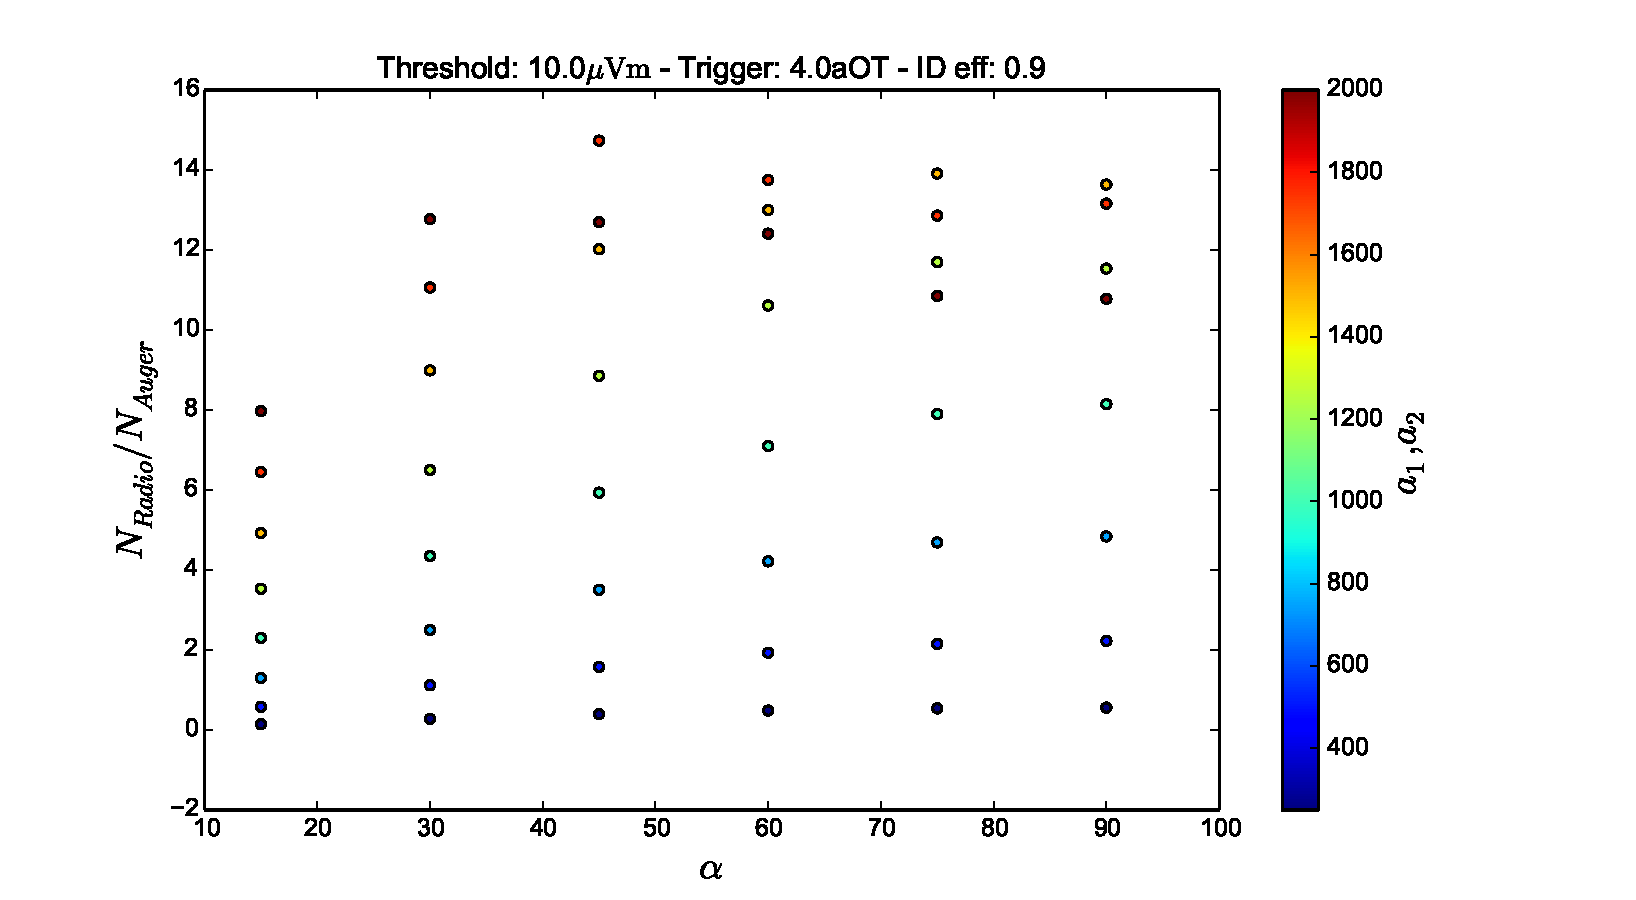
\includegraphics[width=0.7\textwidth]{fig/resultadosRadio/CompRadioAuger_10_0_4_0_0_9_hc_modo1.pdf}
			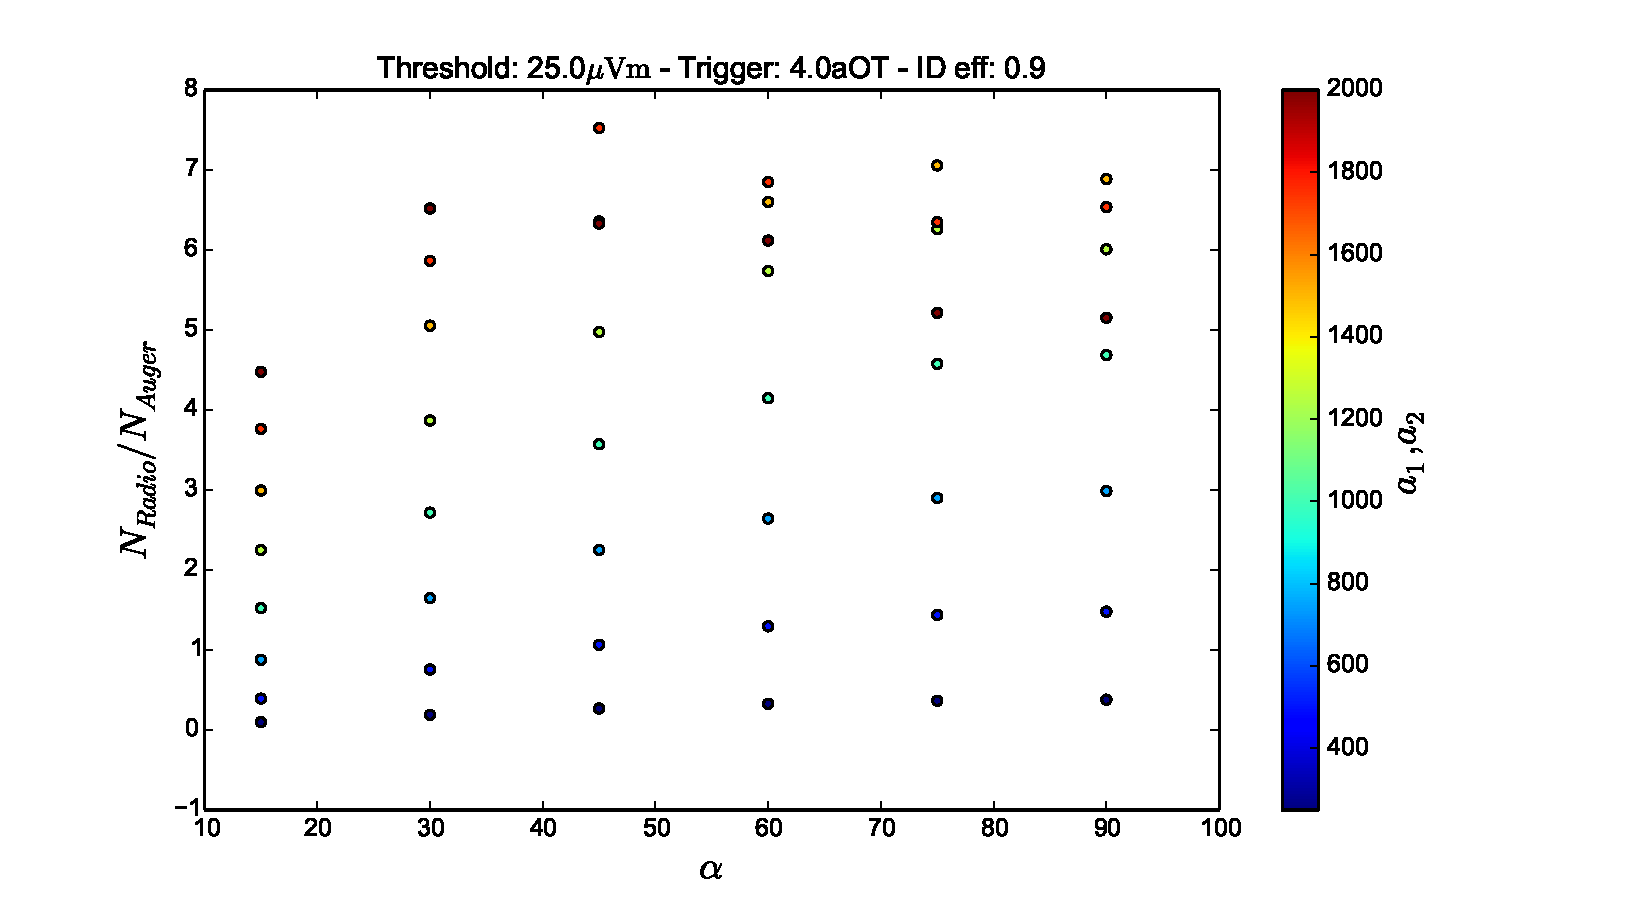
\includegraphics[width=0.7\textwidth]{fig/resultadosRadio/CompRadioAuger_25_0_4_0_0_9_hc_modo1.pdf}
			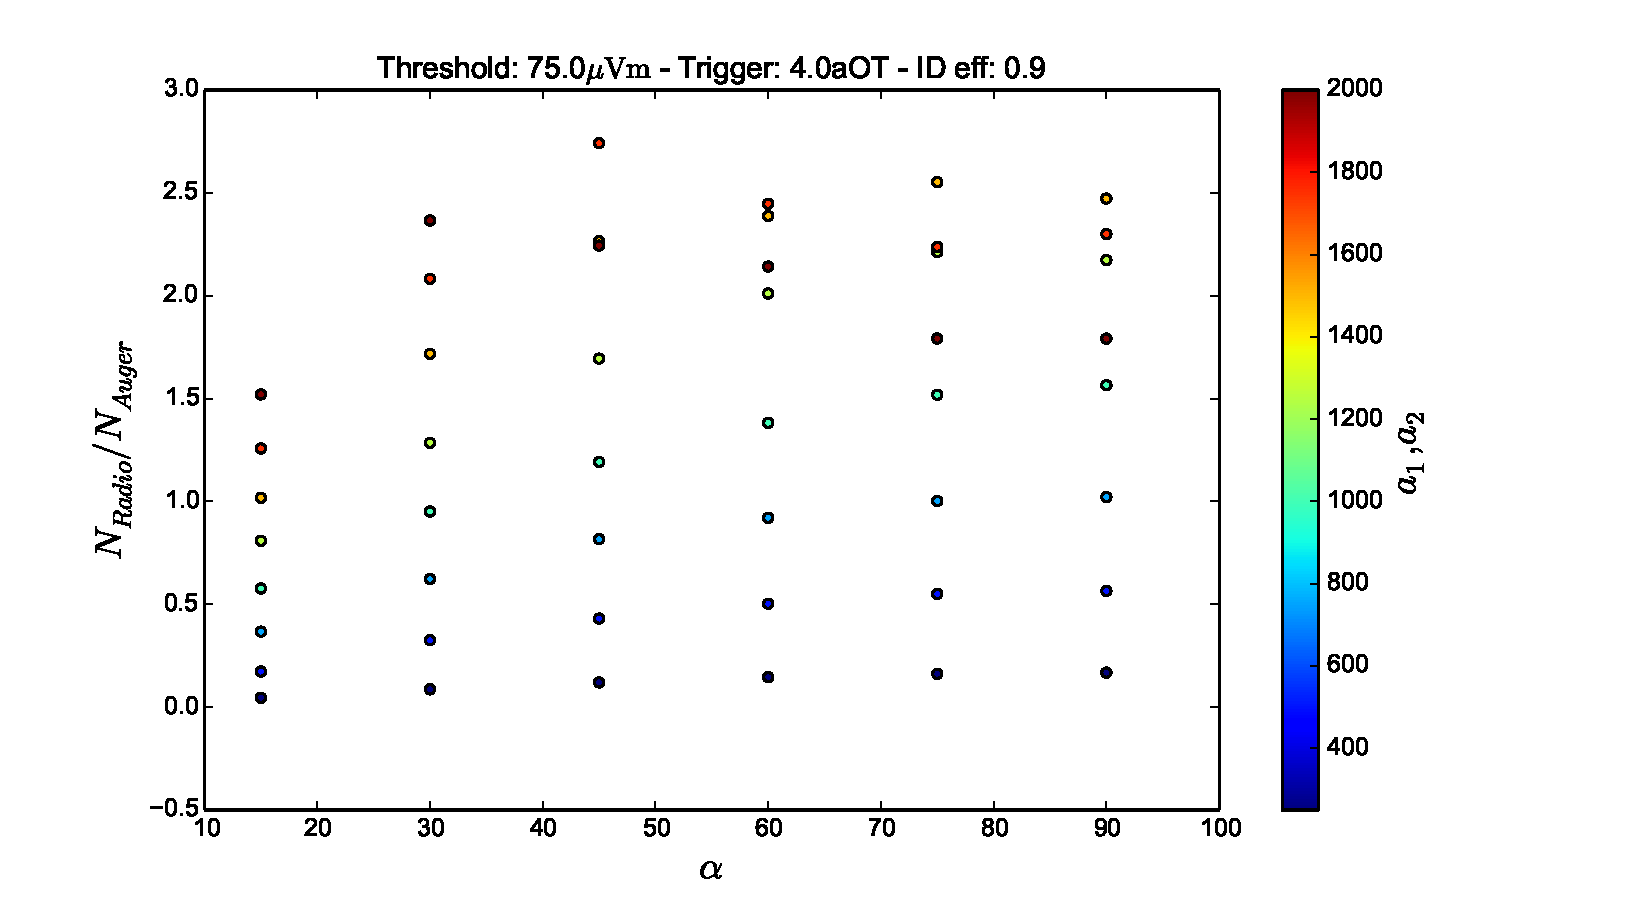
\includegraphics[width=0.7\textwidth]{fig/resultadosRadio/CompRadioAuger_75_0_4_0_0_9_hc_modo1.pdf}
			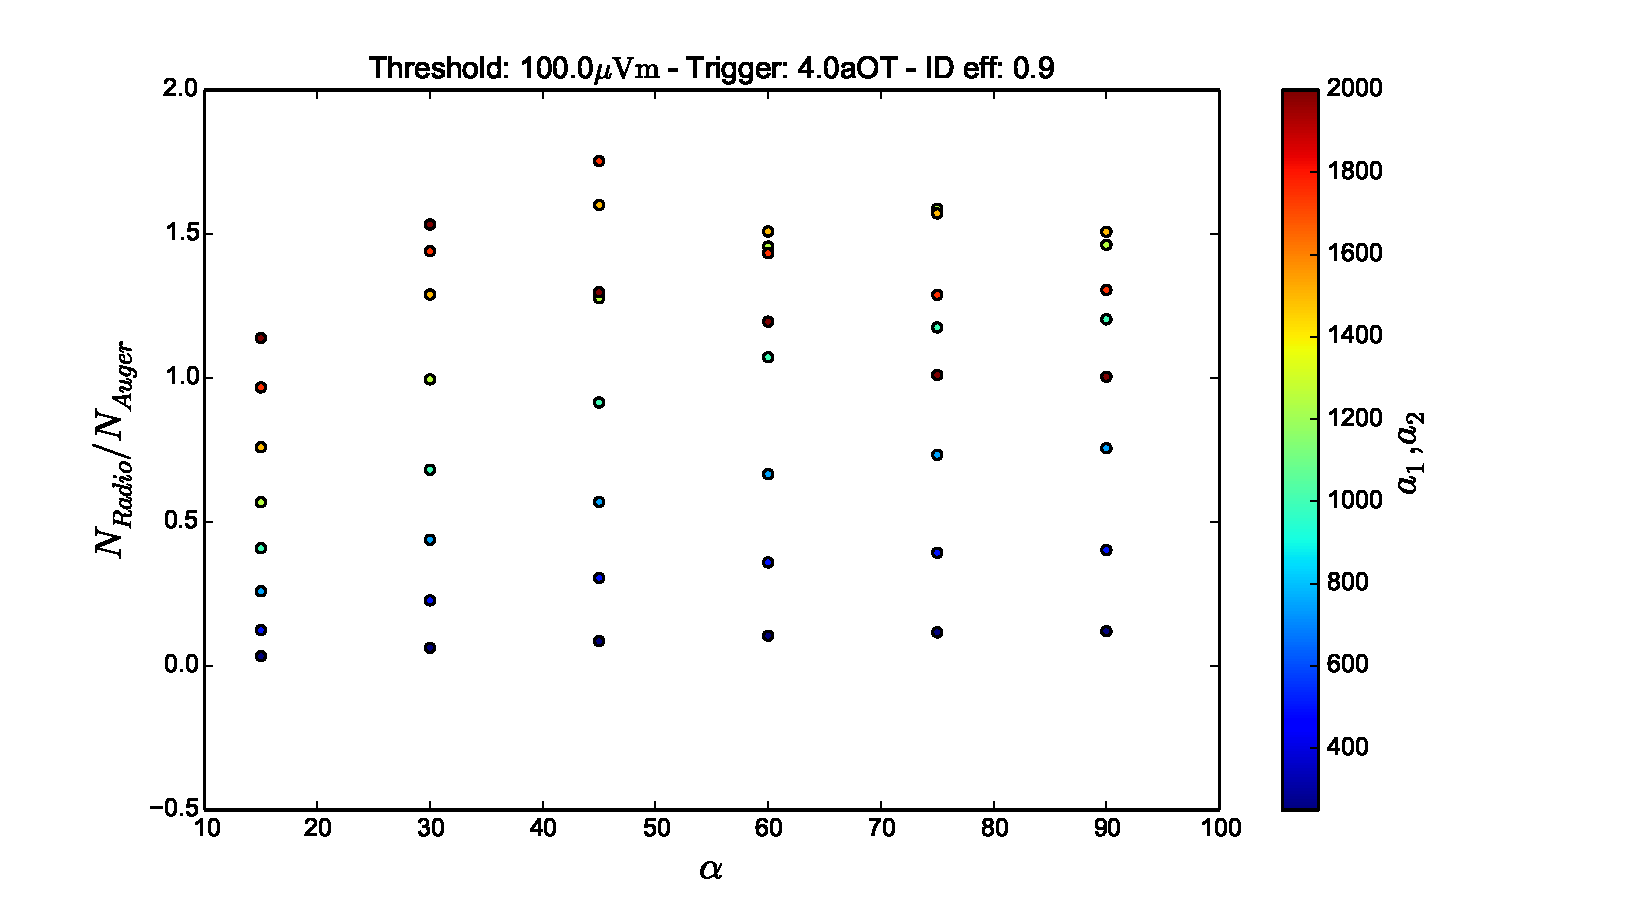
\includegraphics[width=0.7\textwidth]{fig/resultadosRadio/CompRadioAuger_100_0_4_0_0_9_hc_modo1.pdf}
			\caption{asd}
			\label{fig:}
		\end{center}
	\end{figure}
	
	
\section{Un detector de 10000 antenas}

El objetivo de esta secci\'on es discutir la posibilidad de armar un detector de 10000 antenas de radio cuyo fin ser\'ia detectar neutrinos ES.
Para ello, ser\'a necesario utilizar toda la informaci\'on racavada hasta el momento, as\'i como analizar las diferentes topolog\'ias con las que se podrian distribuir 


	\begin{figure}[h!]
		\begin{center}
			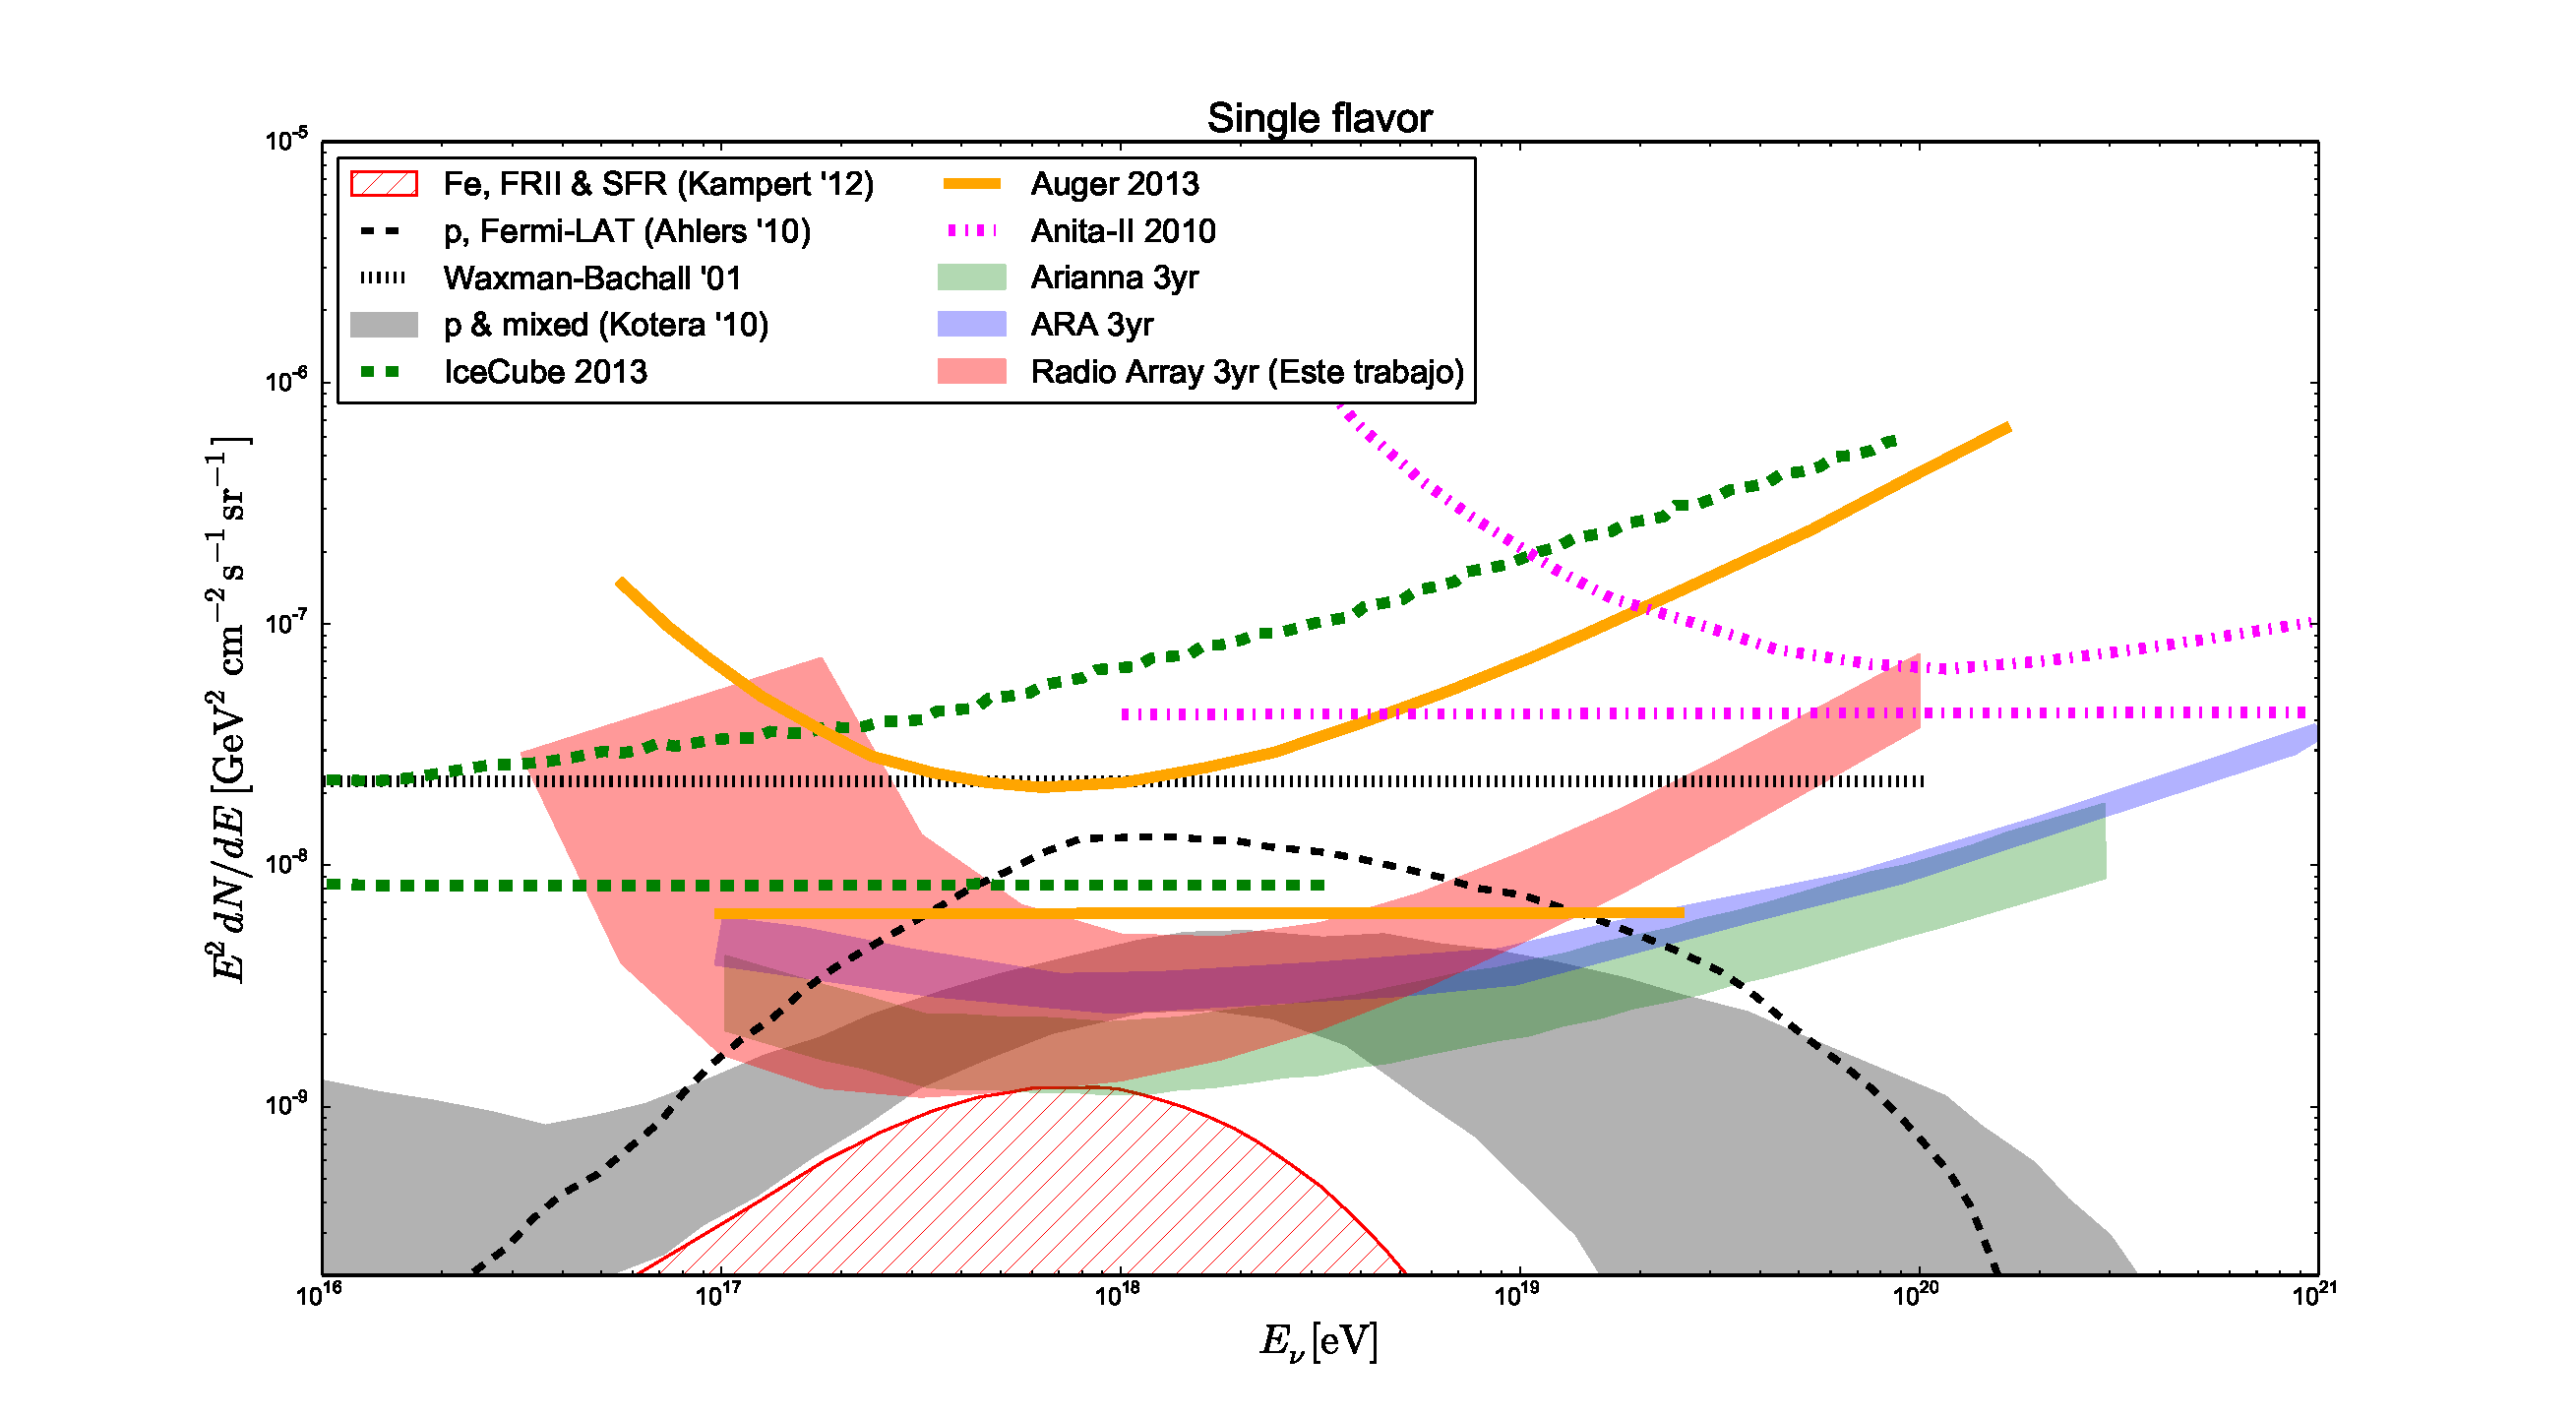
\includegraphics[width=\textwidth]{fig/resultadosRadio/limits_future}
			\caption{asd}
			\label{fig:}
		\end{center}
	\end{figure}